%*
%* Seven Kingdoms: Ancient Adversaries
%*
%* Copyright 1997,1998 Enlight Software Ltd.
%* Copyright 2018 Timothy Rink
%*
%* This program is free software: you can redistribute it and/or modify
%* it under the terms of the GNU General Public License as published by
%* the Free Software Foundation, either version 2 of the License, or
%* (at your option) any later version.
%*
%* This program is distributed in the hope that it will be useful,
%* but WITHOUT ANY WARRANTY; without even the implied warranty of
%* MERCHANTABILITY or FITNESS FOR A PARTICULAR PURPOSE.  See the
%* GNU General Public License for more details.
%*
%* You should have received a copy of the GNU General Public License
%* along with this program.  If not, see <http://www.gnu.org/licenses/>.
%*
%*

\chapter{Seats of Powers and Greater Beings}

\index{seats of power}

\begin{center}
	\textbf{Seats of Power}
	\\ Chinese Greek Mayan Persian Viking
	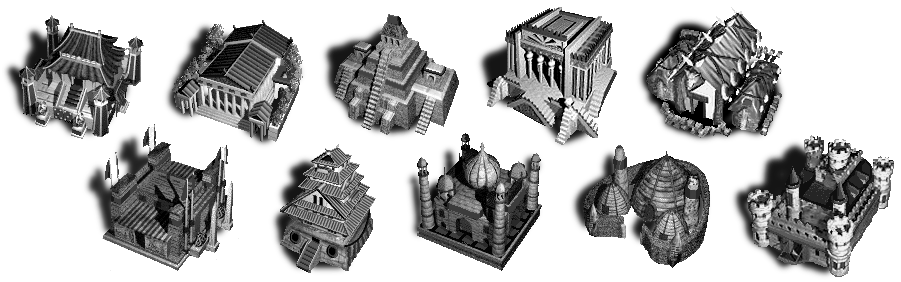
\includegraphics[width=0.7\linewidth]{Iseats}
	\\ Egyptian Japanese Mughul Zulu Norman
\end{center}

\textgoth{\Huge{S}}eats of Power may be built only after a Scroll of Power has been acquired.

They may only be built by Kings, Generals, or trained Construction workers of the appropriate nationality.

A very fortunate Kingdom may end up building seven different Seats of Power, but they may build no more than one of each type.

\clearpage

\section{What purpose do they serve?}

With a Seat of Power, you will be able to Invoke Greater Beings.

Every Nationality has a different Greater Being that it can Summon. These Greater Beings are extremely powerful and versatile---and will either give you good fortune or wreak great havoc on your enemies.

Greater Beings are immune to most of the weapons of mere humans. They are supported by the prayers of the faithful and will only leave this plane when those prayers have been exhausted.

Greater Beings may be invoked again---but only when the prayers have reached an appropriately fevered pitch.

\clearpage % needed for images to fit on the right pages. Graphics here are \linewidth. Needs standard .5 indentation?

\section{Greater Beings}

\subsection{Chinese Jing Nung}

\index{greater beings!Chinese Jing Nung}
\index{Jing Nung}

\begin{center}
	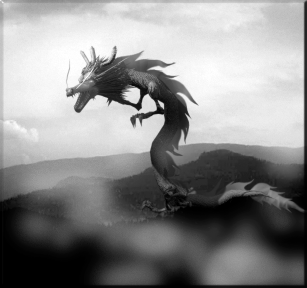
\includegraphics[width=.9\linewidth]{Ajingnung}
\end{center}

\textgoth{\Huge{O}}n your Invocation, the great Jing Nung will appear in the skies over your Chinese Seat of Power.

The Jing Nung will give you clear sight deep into the territory of your foes. If ordered to attack, the Jing Nung’s fire balls will spread flaming death into the ranks of your foes.

You may direct his fire in the same manner as you would for any of your soldiers.

\subsection{Greek Phoenix}

\index{greater beings!Greek Phoenix}
\index{Phoenix}

\begin{center}
	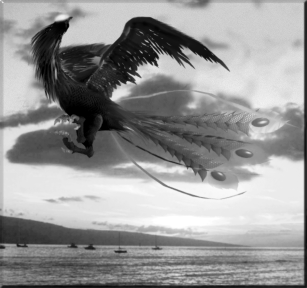
\includegraphics[width=.9\linewidth]{Aphoenix}
\end{center}

\textgoth{\Huge{W}}hen Invoked, the Phoenix will rise from its ashes and appear in the skies over your Greek Seat of Power.

The Phoenix will enable you to see twice as far as the other Greater Beings. In its field of view, it will not only be able to see surface images, but will enable you to gaze into the buildings and Villages of your foes.

You may direct its movements as you do with any of your units.

\subsection{Persian Lord of Healing}

\index{greater beings!Persian Lord of Healing}
\index{Lord of Healing}

\begin{center}
	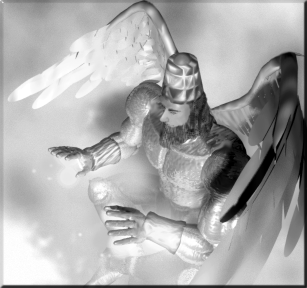
\includegraphics[width=.9\linewidth]{Ahealinglord}
\end{center}

\begin{wrapfigure}{r}{0.1\textwidth}
	\vspace{-20pt}
	\begin{center}
		
\includegraphics[width=.1\textwidth]{Theal}
	\end{center}
	\vspace{-20pt}
\end{wrapfigure}

\textgoth{\Huge{T}}he Lord of Healing will, when you request it, fly over any area of the world and heal all of your people and weapons in that area. To bring this about, direct the Lord of Healing to the appropriate area and \textbf{Click} on the \textbf{Heal Tile}. A large white circle will appear. Center this circle over the target and \textbf{Click} again. Your injured people will be healed of a portion of their wounds.

The healing will affect all units; those outside as well as those inside Ships, Buildings, and Villages. The effect will be stronger, however, on those outside.

\subsection{Norman Dragon}

\index{greater beings!Norman Dragon}
\index{Dragon}

\begin{center}
	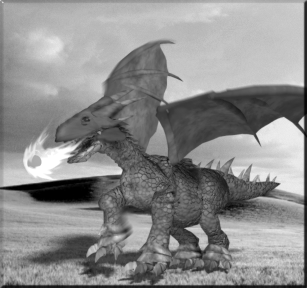
\includegraphics[width=.9\linewidth]{Adragon}
\end{center}

\textgoth{\Huge{W}}hen Invoked, a great Dragon will materialize in the skies over your Norman Seat of Power.

Following your commands, it will fly to the skies over the cities of your foes and strike down with balls of fire. Fear and famine may follow.

A Dragon may be commanded in the same way as you command your common soldiers.

\subsection{Japanese Mind Turner}

\index{greater beings!Japanese Mind Turner}
\index{Mind Turner}

\begin{center}
	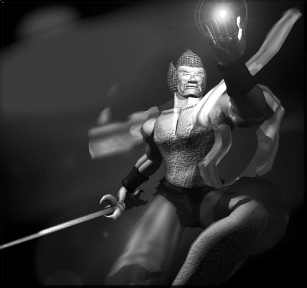
\includegraphics[width=.9\linewidth]{Amindturner}
\end{center}

\begin{wrapfigure}{r}{0.1\textwidth}
	\vspace{-20pt}
	\begin{center}
		
\includegraphics[width=0.1\textwidth]{Tmindturn}
	\end{center}
	\vspace{-20pt}
\end{wrapfigure}

\textgoth{\Huge{T}}he Mind Turner will fly over an enemy area chosen by you. \textbf{Click} on the \textbf{Mind Turning Tile} and center the large white circle over the area where you wish to work your magic. When you \textbf{Click} again, enemy soldiers, workers, and peasants will find themselves less inclined to support their King, sometimes to the point of open revolt.

This power will affect all units; those outside as well as those inside Ships, Buildings, and Villages. The effect will be stronger, however, on those outside.

\subsection{Mayan Kukulcan}

\index{greater beings!Mayan Kukulcan}
\index{Kukulcan}

\begin{center}
	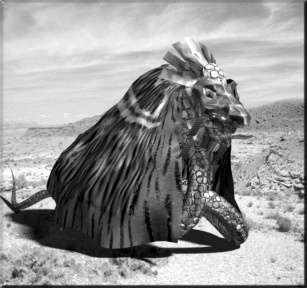
\includegraphics[width=.9\linewidth]{Akukulcan}
\end{center}

\textgoth{\Huge{T}}he Invocation of Kukulcan will grant you the power to greatly increase the fighting skill of your Mayan units.

\begin{wrapfigure}{r}{0.1\textwidth}
	\vspace{-20pt}
	\begin{center}
		
\includegraphics[width=0.1\textwidth]{Tfightupgrade}
	\end{center}
	\vspace{-20pt}
\end{wrapfigure}

To dispense this magic, \textbf{Click} on the \textbf{Fighting Upgrade Tile} and center the large white circle over your target. When you \textbf{Click} again, the transformation shall take place.

The transformation will affect all Mayan units in the area, those outside as well as those inside Ships, Buildings, and Villages. The effect will be stronger, however, on those outside.

\subsection{Viking Thor}

\index{greater beings!Viking Thor}
\index{Thor}

\begin{center}
	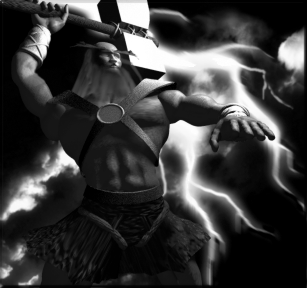
\includegraphics[width=.9\linewidth]{Athor}
\end{center}

\textgoth{\Huge{W}}ith Thor in the skies, your Kingdom will have the power to summon Thunderstorms or Tornadoes. They are so ordered by \textbf{Clicking} on either the \textbf{Thunderstorm Tile} or the \textbf{Tornado Tile} when Thor is over the desired position.

\begin{wrapfigure}{r}{0.1\textwidth}
	\vspace{-20pt}
	\begin{center}
		
\includegraphics[width=0.1\textwidth]{Train}
	\end{center}
	\vspace{-20pt}
\end{wrapfigure}

Thunderstorms are most useful for putting out fires that threaten your buildings and the lives of your people. \\

\begin{wrapfigure}{r}{0.1\textwidth}
	\vspace{-20pt}
	\begin{center}
		
\includegraphics[width=0.1\textwidth]{Ttornedo}
	\end{center}
	\vspace{-20pt}
\end{wrapfigure}

\textgoth{\Huge{T}}ornadoes are best for striking at the heart of your enemy’s Kingdom. When you \textbf{Click} on the \textbf{Tornado Tile}, your cursor will change into a small square. Center this square on your target and \textbf{Click}. Thor will fly to the area and summon a tornado to the spot. When Thor has been invoked at full strength, he should be able to summon three or four tornadoes before he returns from whence he came.

\clearpage

\subsection{Egyptian Isis}

\index{greater beings!Egyptian Isis}
\index{Isis}

\begin{center}
	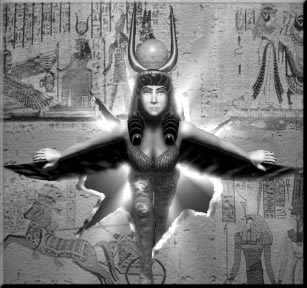
\includegraphics[width=.9\linewidth]{Aisis}
\end{center}

\textgoth{\Huge{T}}he invocation of the fertility goddess Isis will bring the blessings of many healthy children to your villages. Isis can dispense her blessings on any and all nationalities in your Empire.

\begin{wrapfigure}{r}{0.1\textwidth}
	\vspace{-20pt}
	\begin{center}
		
\includegraphics[width=0.1\textwidth]{Tfertility}
	\end{center}
	\vspace{-20pt}
\end{wrapfigure}

When Isis is selected, \textbf{Click} on the \textbf{Fertility Tile} and then place the small white square over one of your Villages and \textbf{Click}. When you do, Isis will fly to the location and work her magic. The population of the selected Village will increase by five for every Click.

\subsection{Mughul Djinni}

\index{greater beings!Mughul Djinni}
\index{Djinni}

\begin{center}
	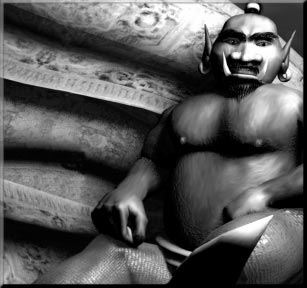
\includegraphics[width=.9\linewidth]{Adjinni}
\end{center}

\textgoth{\Huge{T}}he Djinni is the spirit of the desert winds who strikes fear into the hearts of those who would dare to oppose you. This fear will cause enemy people to harbor resentment against their King, even to the point of betrayal.

\begin{wrapfigure}{r}{0.1\textwidth}
	\vspace{-20pt}
	\begin{center}
		
\includegraphics[width=0.1\textwidth]{Tdjinni}
	\end{center}
	\vspace{-20pt}
\end{wrapfigure}

When the Djinni is selected, \textbf{Click} on the \textbf{Djinni Tile} and then place the small white square over your intended target. This target may be any soldier, worker, or peasant of the enemy who has been caught out of doors. The Djinni will have no effect on those cowering inside their Village houses.

The decrease of a target's loyalty will be between 20 and 30 points for each Click.

\subsection{Zulu uNkulunkulu}

\index{greater beings!Zulu uNkulunkulu}
\index{uNkulunkulu}

\begin{center}
	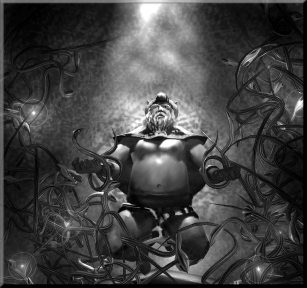
\includegraphics[width=.9\linewidth]{Aoldone}
\end{center}

\textgoth{\Huge{u}}Nkulunkulu, the “Old, Old One” of the Zulus, can be called from his abode to give great leadership skills to your Zulu Generals.

\begin{wrapfigure}{r}{0.1\textwidth}
	\vspace{-20pt}
	\begin{center}
		
\includegraphics[width=0.1\textwidth]{Toldone}
	\end{center}
	\vspace{-20pt}
\end{wrapfigure}

When uNkulunkulu has been invoked and selected, \textbf{Click} on the \textbf{Shield and Assegai Tile}. Then place the small white box over your targeted Zulu General. For each Click thereafter, the General will gain 30 points in Leadership skill. This magic will work only on Zulu Generals, not on common soldiers and not on the people of any other race.

\section{How to Invoke a Greater Being}

\index{invoking greater beings}

\textgoth{\Huge{O}}nce you have recovered a Scroll of Power and built a Seat of Power, you must assign a General or your King to it. It is he who will lead the prayers of the faithful.

The faithful are the people that you have sent into the Seat of Power just as you would send people into a Mine or Factory.

You may send in up to 8 units---of the appropriate Nationality only. These units must be Peasants or units who already possess Praying skills. Other units are unacceptable---as their education has cluttered their minds.

As these people enter the Seat of Power, they will immediately begin their prayers to the Greater Being. You need do nothing but wait.

While they are in the Seat of Power, their skill in Praying will gradually increase. The speed of the increase will depend upon the leadership level of the commander in the Seat of Power.

If the those praying are sent out of the Seat of Power, they will retain their skill and show the Praying icon over their heads.

\begin{wrapfigure}{r}{0.1\textwidth}
	\vspace{-20pt}
	\begin{center}
		
\includegraphics[width=0.1\textwidth]{Tinvoke}
	\end{center}
	\vspace{-20pt}
\end{wrapfigure}

% GENDER HERE.

Once the prayers have reached the minimum level of 40 points out of the maximum of 400, you may Invoke the Greater Being by \textbf{Clicking} on the \textbf{Invoke Tile}.

This being done, the Greater Being will appear hovering over your Seat of Power, ready to listen to your request as to what he or she should do. You may direct him or her as you would an ordinary being.

Upon Invocation, the Greater Being will begin consuming the Pray Points in the Seat of Power. He or she will use very little if left alone, but when his or her spells are cast, he or she will use up a good portion.

These Pray Points are the exact equivalent of the Hit-Points of ordinary units, and so when the Pray Points have been exhausted, the Greater Being will disappear. You may of course Invoke him or her again at a later date.

Greater Beings may not be injured by mere mortals.

If you have captured an enemy’s Seat of Power, you will be able to use it to invoke Greater Beings. You will not, however, acquire the Scroll of Power and the knowledge required to build another Seat of Power of the same kind.
